
\documentclass[12pt]{article}
\usepackage[T2A]{fontenc}
\usepackage[english,russian]{babel}
\usepackage[utf8]{inputenc}
\usepackage{graphicx,articleStyle}
\pagestyle{fancy} 
\fancyhead{} 
\fancyfoot{} 

\linespread{1.0}

\usepackage{amsmath}
\usepackage{multirow}
\makeatletter
\fancyhead[RO]{\small Конфигурационное управление \\ {11.12.2022} }
\fancyhead[LO]{\small Применение Agile Scrum в проектах SAP}

\c@page=1 
\makeatother

% Название доклада на русском языке:
\title{Применение Agile Scrum в проектах SAP}

\author{\small Степанов Дмитрий Юрьевич \\ \small Вельсовский Андрей Вельтерович } 

\email{\small mail@stepanov.com \\ \small velsovskiyav@mail.ru}

\begin{document}

\udk{Пример УДК}

{\let\newpage\relax\maketitle}

\vskip -1.5em

\begin{abstract}
Работа содержит описание метода Agile Scrum в проектах внедрения корпоративных информационных 
систем на базе SAP. Рассматриваются вопросы применения Scrum в проектах развития, тиражирования 
и внедрения <<с нуля>> решений SAP, а также использования гибкой методологии Agile для 
разработки и кастомизации информационных систем. Сделан вывод о целесообразности применения метода
Scrum в проектах развития SAP-систем путем доработки
\keywords{\emph{Agile, Scrum, SAP, информационные системы}}
\end{abstract}
%%%%%%%%%%%%%%%%%%%%%%%%%%%%%%%%%%%%%%%%%%%%%%%%%%%%%%%%%%%%%%


\section{Введение}
Пожалуй, нет более популярной темы для обсуждения, чем применение Agile в проектах SAP. Несмотря
на то, что принципы гибкой разработки были сформулированы еще в 2001 году \cite{LarmanC}, их 
использование в настоящее время становится как никогда востребованным. Связано это в первую очередь
с тем, что последнее десятилетие знаменуются массовым использованием информационных технологий (далее - ИТ)
в повседневной жизни: порталы государственных услуг, интернет-магазины, электронные правительство и 
многое другое. Вышесказанное требует как грамотной программного обеспечения (далее - ПО), так и не 
менее искусного его внедрения.

\section{Agile - гибкая методология разработки }
\subsection{Agile Scrum}

\begin{figure}
  \centering
  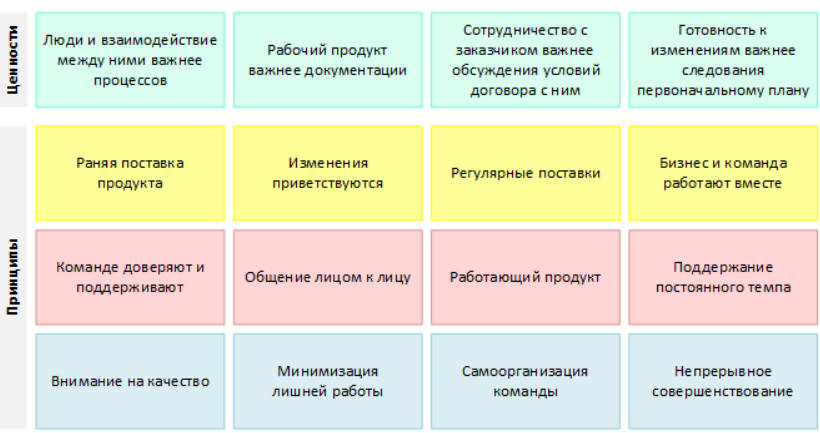
\includegraphics[width=1\textwidth]{./figures/AgilePrinciples.png}
  \caption{\label{fig:agilePrinciples}Ценности и принципы Agile}
\end{figure}

Agile представляет собой методологию реализация и внедрения ПО на основе итерационной модели и включает
совокупномть методов, к которым можно отнести FDD (Feature Driven Delevopment - разработка, управляемая 
функциональностью), XP (eXtreme programming - экстремальное программирование), Kanban, Crystal и др. 
Суть методолгии заключается в использовании 4 базовых ценностей и 12 принципов (рис. \ref{fig:agilePrinciples}) , 
объявленных в манифесте Agile \cite{agileManifest}, следование которым призвано существенно облегчить имплементацию 
информационных систем (далее -ИС). Одним из ярких примеров использования принципов Agile является метод Scrum 
Рассматриваемый как противовес классической каскадной модели (Waterfall - водопадная модель) внедрения ИС, 
метод Scrum дает четкое представление процесса имплементации и описывает реализацию базовых составляющий 
манифеста. Справедливости ради следует отметить, что Scrum частично применяется и в водопадной модели, например,
для уточнения требований на фазе анализа путем прототипирования.

\begin{figure}
  \centering
  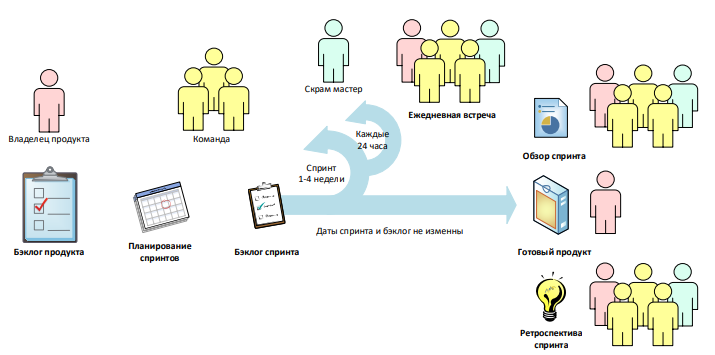
\includegraphics[width=1\textwidth]{./figures/ScrumRealizationChart.png}
  \caption{\label{fig:scrumRealizationChart}Процесс реализации проекта согласно Scrum}
\end{figure}

\subsection{Итерации Scrum}

Напомним, итеративный подход реализации ПО заключается в разбиении процесса внедрения на стадии, называемые итерациями, 
в рамках которых разрабатывается и демонстрируется заказчику реализованная часть решения \cite{InfoSysImplementation}. При этом 
как таковые требования вообще могут отсутствовать, количество предстоящих итераций неизвесто, а объем
проекта изменяем при фиксированных сроках и бюджет. Следуя методу Scrum, итерация называют спринтами, список 
требований - бэклогом (Backlog), ход проекта контролируют на доске стикерами, а команда рассматривается как 
самоорганизующаяся \cite{AgilePrinciples}. Концептуальная картина ведения проекта имплементации согласно Scrum дана выше 
на рис. \ref{fig:scrumRealizationChart}

\subsection{Подтверждение работоспособности ИС}

Несмотря на отличие каскадной и итерационной моделей внедрений ИС, обеих подходах подтверждением 
работоспособности разработанной системы служит успешное пройденное приемочное тестирование (User Acceptance Test - UAT)\cite{InfoSysImplementation}. 
Однако метод Scrum существенно отличается от обеих из-за отсутствия UAT и документирования решения. Проект 
внедрения корпоративных информационных систем (далее - КИС) с использованием Scrum состоит из следующих шагов:

\begin{itemize}
\item идентификаия и аналз требований, предъявляемых к КИС, приоритизация найденных требований и формирование бэклога продукта;
\item определение числа продолжительности спринтов разработки КИС;
\item формирование бэклога спринтов и их распределение по итерациям;
\item реализация КИС согласно бэклогу спринта, функциональное интеграционное тестирование, демонстрация 
полученного результата владельцу продукта и заказчику, ретроспектива спринта и обновление бэклогов, а также
продуктивная эксплуатация реализованного решения (для всех спринтов\cite{AgilePrinciples}).
\end{itemize}

Более того, в отличие от каскодной и итерационной моделей, мерилом реализации проекта Scrum является спринт (часть продукта),а не продукт.
Так в Scrum промышленному использованию подлежит результат каждого спринта, даже если финальный спринт, обозначающий 
реализацию всего продукта, еще не реализован.

\subsection{Кастомизация и настройка ИС}

Методология Agile изначально была ориентирована на разработку, но не на кастомизацию ПО, 
именно поэтому под Scrum-командой понимается состав из 5-7 разработчиков. Кастомизация 
представляет собой настройку ИС, не требующую программной доработки решения. Настройка ПО 
ведётся силами функциональных консультантов, в то время как реализация решения – программными
разработчиками. Следует отметить, что число вариаций настроек системы под нужды заказчика 
весьма ограничено. Кастомизация ИС обеспечивает стандартизацию, унификацию, а также прозрачность 
решения: новичку гораздо проще разобраться в настройках в виду их детерминированности, нежели с 
программными разработками. Допустим, кастомизация ведётся силами разработчиков. Современные 
корпоративные информационные системы, например, от компании SAP AG: ERP, SRM, SRM и другие,
функционируют и претерпевают изменения из-за:

\begin{itemize}
  \item внедрения <<с нуля>>;
  \item тиражирования;
  \item развития.
\end{itemize}

\begin{flushleft}
  а проект внедрения характеризуется функциональными:
\end{flushleft}
 
\begin{itemize}
  \item большим объемом основных и переменных данных для целей миграции и последующего использования в SAP;
  \item единой интегрированной организационной структорной предприятия в SAP;
  \item заданным числом бизнес-процессов для отражения в SAP;
  \item большим массивом транспортных запросов и задач переноса в SAP.
\end{itemize}

\begin{flushleft}
  и организационными особенностями:
\end{flushleft}
 
\begin{itemize}
  \item большим числом членов проектной команды ( в зависимости от проекта - 1-5 человек в рамках одного функционального
        направления, в проекте может быть от 1 до 7 направлений);
  \item интеграцией SAP с внешними системами.
\end{itemize}


\section{Внедрение систем, реализованных согласно методу Agile-Scrum}
\subsection{Оценка целесообразности внедрения}
Внедрение подобных систем осуществляется преимущественно на основе каскадной модели в виду 
дороговизны, объёмности, сложности и продолжительности проекта. Проделаем следующее упражнение: 
выделим способы реализации КИС, а также виды проектов, далее для пары «способ-вид» попытаемся 
эмпирически оценить целесообразность использования Agile Scrum (табл. \ref{tab:expediencyOfUsingAgileScrum}). В качестве оценивания 
выберем шкалу от 1 до 3, где 1 – применение маловероятно, 2 – использование возможно, но 
требуется значительная трансформация команды, 3 – рекомендуется использовать Scrum.

\vskip 1.5em

\begin{table}[h!]\begin{center}
  \caption{Целесообразность применения Agile Scrum в проектах SAP}\label{tab:expediencyOfUsingAgileScrum}
  \begin{tabular}{|p{4cm}|p{3cm}|p{4cm}|}
    \hline
    Способ реализации & Вид проекта & Целесообразность \\ \hline
    Разработка & Развитие & 2-3 \\ \hline
    Настройка & Развитие & 1-2 \\ \hline
    Настройка и разработка & Внедрение <<с нуля>>, тиражирование & 1 \\ \hline 
  \end{tabular}
\end{center}\end{table}

\subsection{Требования к проектной команде} 

% subsection subsection_name (end)
Использование Agile Scrum для доработки SAP системы в процессе ее разваития действительно может позволить достичь положительного эффекта. Стоит отметить, что разработка затрагивает лишь ограниченный функционал SAP-системы, сравнимый по объему с модулем, например, закупки, сбыт и др.

Применение Scrum диктует особые требования к организации и составу команды:
теперь архитектурные решения должны приниматься доверительно и коллективно;
разработка ведётся от требований, проектные решения, спецификации на разработку и
прочая документация отсутствуют; каждый ежедневно отчитывается о результатах
проделанной работы. Для использования гибкой методологии необходима
трансформация проектной команды, первая попытка которой может закончиться
неудачей. Преимущества Scrum будут ощутимы только при условии, что команда
непрерывно работает над проектами, используя гибкую методологию Agile, а не от
случая к случаю: применение Scrum требует преодоления инерции водопадной
модели. Одно и тоже требование может быть одновременно неправильно трактовано и
неверно реализовано, непрерывная демонстрация разрабатываемого решения
владельцу продукта и конечным пользователям позволяет получить именно тот
результат, который ожидает и хочет увидеть пользователь. В этом заключается
преимущество итерационной модели, к которой относится и Agile. Таким образом,
целесообразность использования Agile Scrum в проектах развития SAP-систем за счёт
их доработки видится оправданной, однако требует значительных изменений в
мышлении, организации и понимании новых правил игры всей проектной команды
(табл. \ref{tab:expediencyOfUsingAgileScrum}, оценка целесообразности 2-3).

\subsection{Внедрение SAP}
Обратимся к случаю кастомизации системы SAP в процессе ее развития. Самый простой 
пример - внедрение ранее не использованного модуля, например, SAP ERP WM 
(Warehouse Managment - управление складами). Подобные активности не требуют чрезмерных 
трудозатрат функицонального консультанта. Давайте разберемся за счет чего достигается 
положительный эффект применеия Scrum в процессе доработки SAP. Программа может быть 
организована и запрограммирована огромным числом способов, гибкая модель разработки 
позволяет выбрать лишь тот, который удовлетворяет конечному пользователю. В случае 
настройки SAP-системы ситуация в корне иная: кастомизация решения весьма ограничен, 
а варианты настройки либо носят единичный характер, либо очень близки. 
Демонстрация промежуточного продукта пользователю кардинально не может изменить 
выбранного решения в виду его детерминированности. В итоге, конечный пользователь мало на что может
повлиять, а сам метод Scrum обеспечивает лишь быструю доставку решения без
какой-либо существенной обратной связи (табл. \ref{tab:expediencyOfUsingAgileScrum}, оценка целесообразности 1-2).

И, наконец, полномасштабное внедрение SAP. Значительная часть проектов как
тиражирования, так имплементации SAP «с нуля» требует доработки: кастомизация в
большинстве своём не может покрыть всех требований бизнеса. Начнём с 
организационных сложностей: проект внедрения SAP требует вовлечения большого
числа как разработчиков, так и консультантов. В зависимости от проекта количество
членов команды может варьироваться от 5 до 37, что явно нарушает требования Scrum
(согласно гибкой методологии команда должна состоять из 5-7 разработчиков).
Практически каждый проект SAP включает интеграцию с внешними системами. Вне
зависимости от содержания и качества реализации спринтов проектной командой
SAP, велика зависимость от внешнего ресурса. Игнорирование плана проекта SAP,
задерживание тестирования и выпуска продукта, не информирование о внесённых
изменениях и прочие действия внешней стороны критически влияют на выполнение
спринта и не могут быть устранены в рамках Scrum.

\subsubsection{Функциональные требования SAP} % (fold)
% subsubsection subsubsection_name (end)

Перейдём к функциональным особенностям. SAP-система представляет собой
интегрированную среду, объединяющую данные, организационную структуру и
процессы компании. Все три указанных звена являются общими и каждое из
функциональных направлений может вносить свои изменения, поэтому спринты
должны организовываться кросс-командно, что весьма нетривиально. Разумнее всего в
число первых спринтов включить заведение организационной структуры, являющейся
основополагающей частью предприятия. В последующих спринтах следует
позаботиться о миграции и ведении основных и переменных данных для всех
направлений бизнеса. И лишь потом сосредоточиться на реализации бизнеспроцессов. Важно заметить, что всё вышеперечисленное ведётся в системе SAP
настройками, за исключением, пожалуй, процессов, требующих значительной
доработки. Тем самым, применение Scrum целесообразно только для реализации
бизнес-процессов SAP, в то время как для организационной структуры и данных
гибкая методология позволяет выполнить лишь демонстрацию и исправление
очевидных ошибок.

\subsection{Agile Scrum и SAP-продукты}

И последнее, Agile Scrum анонсирует принцип регулярных поставок за счёт
использования фич (Feature - переключатель). Тем самым реализованные программы
переносятся в продуктивную среду по мере выполнения спринтов, включение и
отключение внесённых изменений обрабатывается переключателями, чтобы не
навредить существующим разработкам. К доработкам SAP вопросов нет, но как быть с
настройками, ведь механизм переключателей здесь не работает? Более того,
выполнив одну настройку, можно изменить другую, в модификации которой не было
необходимости. Можно подумать о реализации дополнительных программ,
выполняющих функции переключателей к настройкам, однако в SAP так много
позиций кастомизации, что доработка выльется в неоправданно большие затраты
Авторы должны представить в оргкомитет PDF-файл статьи, оформленной по данному шаблону. 

\begin{table}[h!]\begin{center}
  \caption{Особенности проекта SAP с точки зрения Scrum}\label{tab:SapScrumSpecifications}
  \begin{tabular}{|p{4cm}|p{2.5cm}|p{5cm}|}
    \hline
    Особенность & Соответствие Agile Scrum & Комментарий \\ \hline
    Число участников проектной команды & Нет & Число участников много больше \\ \hline
    Интеграция с внешними системами & Нет & Scrum не устраняет риски внешних сторон \\ \hline
    Данные,  & \multirow{2}{*}{Нет}& \multirow{2}{5cm}{Быстрая доставка без возможности существенных изменений}   \\
    Организационная структура &                             &                                         \\ \hline
    Бизнес-процессы  & Да & Быстрая доставка с обратной связью \\ \hline
    Транспортные запросы & Нет & Перенос в продуктивную систему только запросов разработки, но не настройки \\ \hline
  \end{tabular}
\end{center}\end{table}

\section{Итоги внедрения Scrum в SAP-проекты}
Подведём небольшой итог применения Scrum в больших проектах SAP,
требующих как кастомизацию, так и разработку системы. Результаты обсуждения
функциональных и организационных особенностей проекта SAP вынесены в табл. 2.
Из данных таблицы можно сделать следующий вывод: значительное преимущество
Scrum вносит только с точки зрения реализации бизнес-процессов, все прочие
аспекты проекта существенно не улучшаются. Таким образом, использование Agile
Scrum в проектах тиражирования и внедрения SAP «с нуля» выглядит весьма спорно
(табл. 1., оценка целесообразности 1).
Вернёмся ещё раз к каскадной модели внедрения SAP. Возьмём манифест Agile
\cite{ScrumSap} и попытаемся понять, насколько он покрывается водопадной моделью. Получим
следующие результаты:

\begin{itemize}
  \item принципы совместной работы команды и минимизации лишней работы
отражены в модели водопад за счёт вовлечения ключевых пользователей и
выполнении только включённых в объём проекта работ;
  \item принципы общения лицом к лицу и внимания к качеству находят частичное
покрытие в каскадной схеме внедрения КИС;
  \item все прочие принципы и ценности Agile не релевантны в каскадной модели.
\end{itemize}

Разберёмся, почему в модели Waterfall применяется так мало принципов Agile.
Возможно от того, что в каскадной схеме внедрения КИС акцент сделан на иные
сущности. Проведём анализ типовых рисков проекта, идентифицированных Б. Бэмом.
при усовершенствовании итерационной и создании спиралевидной модели \cite{InfoSysImplementation}.
Сгруппировав риски, выделим проблемные области имплементации КИС

\begin{itemize}
  \item нереальность сроков, бюджета, а также дефицит ресурсов проекта;
  \item технические недоработки и постоянные изменения;
  \item участие внешних сторон;
  \item низкая квалификация кадров.
\end{itemize}

Это позволяет сформулировать следующий вывод: метод Agile Scrum нацелен на
решение технических проблем, возникающих в условиях непрекращающихся
изменений, все прочие проблемы проекта вне Scrum. Таким образом, Agile Scrum
хорош с точки зрения разработки программ, когда содержание продукта неизвестно ни
проектной команде, ни пользователям. Однако применение Scrum требует глобальных
изменений в организации проекта и не снижает прочих рисков неудачи.

При имплементации масштабных SAP решений, когда объём проекта понятен
даже при отсутствии детализированных требований, технические неточности
устраняются на этапах системного, интеграционного и приёмочного тестирований.
Agile Scrum существенных преимуществ здесь дать не может, так же как и в случае,
когда затраты на реорганизацию команды и следование Scrum значительно
превосходят цикл разработки программного решения. Резюмируя вышесказанное,
хочется отметить, что метод Scrum как разновидность итерационной модели
ориентирован в большей степени на пользователей и разработчиков, в то время как
каскадная схема – на руководителей проектов.
%Возможно использовать bibtex.
\bibliographystyle{alpha}
\bibliography{sample}


\end{document}
